\documentclass[12pt]{article}

\usepackage[utf8]{inputenc}
\usepackage{geometry}
\geometry{a4paper,scale=0.75}
\linespread{1.5}
\usepackage{graphicx} 
\usepackage{float} 
\usepackage{subfig} 
\usepackage{enumerate}
\usepackage{enumitem}
\usepackage{amsmath}
\usepackage{array}
\usepackage{booktabs}
\usepackage{multirow}
\usepackage{amsfonts}
\usepackage[english]{babel}
\usepackage{amsthm}
\usepackage{dcolumn}
\usepackage{multicol}
\usepackage{stfloats}
\usepackage{lscape}
\usepackage[figuresright]{rotating}
\RequirePackage{pdflscape}
\usepackage[toc,page]{appendix}
\usepackage{geometry}
\usepackage{longtable}
\usepackage{comment}
\usepackage{xcolor}

% -------- enumerated sub-labels (a), (b), … --
\usepackage{enumitem}
\setlist[enumerate,1]{label=(\alph*),ref=\alph*}
% ---------------------------------------------

\usepackage{hyperref}
\hypersetup{hidelinks,
	colorlinks=true,
	allcolors=black,
	pdfstartview=Fit,
	breaklinks=true}
\usepackage{csquotes}
\usepackage{natbib}
\bibliographystyle{apalike}
\newtheorem{definition}{Definition}
\newtheorem{theorem}{Theorem}
\newtheorem{proposition}[theorem]{Proposition}
\newtheorem{lemma}[theorem]{Lemma}
\newtheorem{corollary}[theorem]{Corollary}
\newtheorem*{remark}{Remark}
\newtheorem{example}{Example}
\newtheorem{exercise}{Exercise}
\newtheorem{assumption}{Assumption}[section] % number within sections


\begin{document}

\begin{center}
    ECON 3123: Macroeconomic Theory I\\
    {\large \textbf{Tutorial Note 8: IS-LM-PC Framework}}\\
    Teaching Assistant: Harlly Zhou
\end{center}

\subsection*{Deriving the PC Relation}
To put IS-LM and PC together, we need either interest rate or output appear in the PC relation. By this, we mean that we would like to derive a step further from the Phillips curve so that, obviously easier to show, output appears.

Recall that the production function is
\[Y_t = A N_t,\]
where $Y_t$ is the output, $A$ is the productivity, and $N_t$ is the labour force, and that unemployment rate $u_t$ is defined to be
\[u_t = \frac{L-N_t}{L},\]
where $L$ is total labour force minus discouraged worker.
Hence,
\[u_t = 1-\frac{1}{A}\frac{Y_t}{L} \iff Y_t = AL(1-u_t).\]
We can thus define \textbf{the natural level of employment}, $N_n$, and \textbf{the natural level of output}, $Y_n$:
\[N_n = L(1-u_n),\,\, Y_n = AL(1-u_n),\]
where $u_n$ is the natural rate of unemployment.

Then we can rewrite the Phillips Curve equation to obtain the \textbf{PC relation}:
\begin{align*}
    \pi_t - \pi_t^e &= -\alpha (u_t - u_n)\\
    &= -\alpha\left[\left(1-\frac{1}{A}\frac{Y_t}{L}\right) - \left(1-\frac{1}{A}\frac{Y_n}{L}\right)\right]\\
    &= \frac{\alpha}{AL}(Y_t - Y_n).
\end{align*}

Figure \ref{fig:pc01} demonstrates how a PC curve looks like in a $(Y, \pi-\pi^e)$ diagram. From the mathematical formulation, we know that the line must pass $(Y_n,0)$. This is supported by economics: when the market is in medium-run equilibrium, inflation expectation matches the true inflation, and the output is at the natural level. Let $\pi^e=\bar{\pi}$, the targeted inflation. Then in this diagram, the corresponding output $Y_t$ is larger than the natural level. In this case $N_t > N_n$, and $u_t < u_n$.
\begin{figure}[htp]
    \centering
    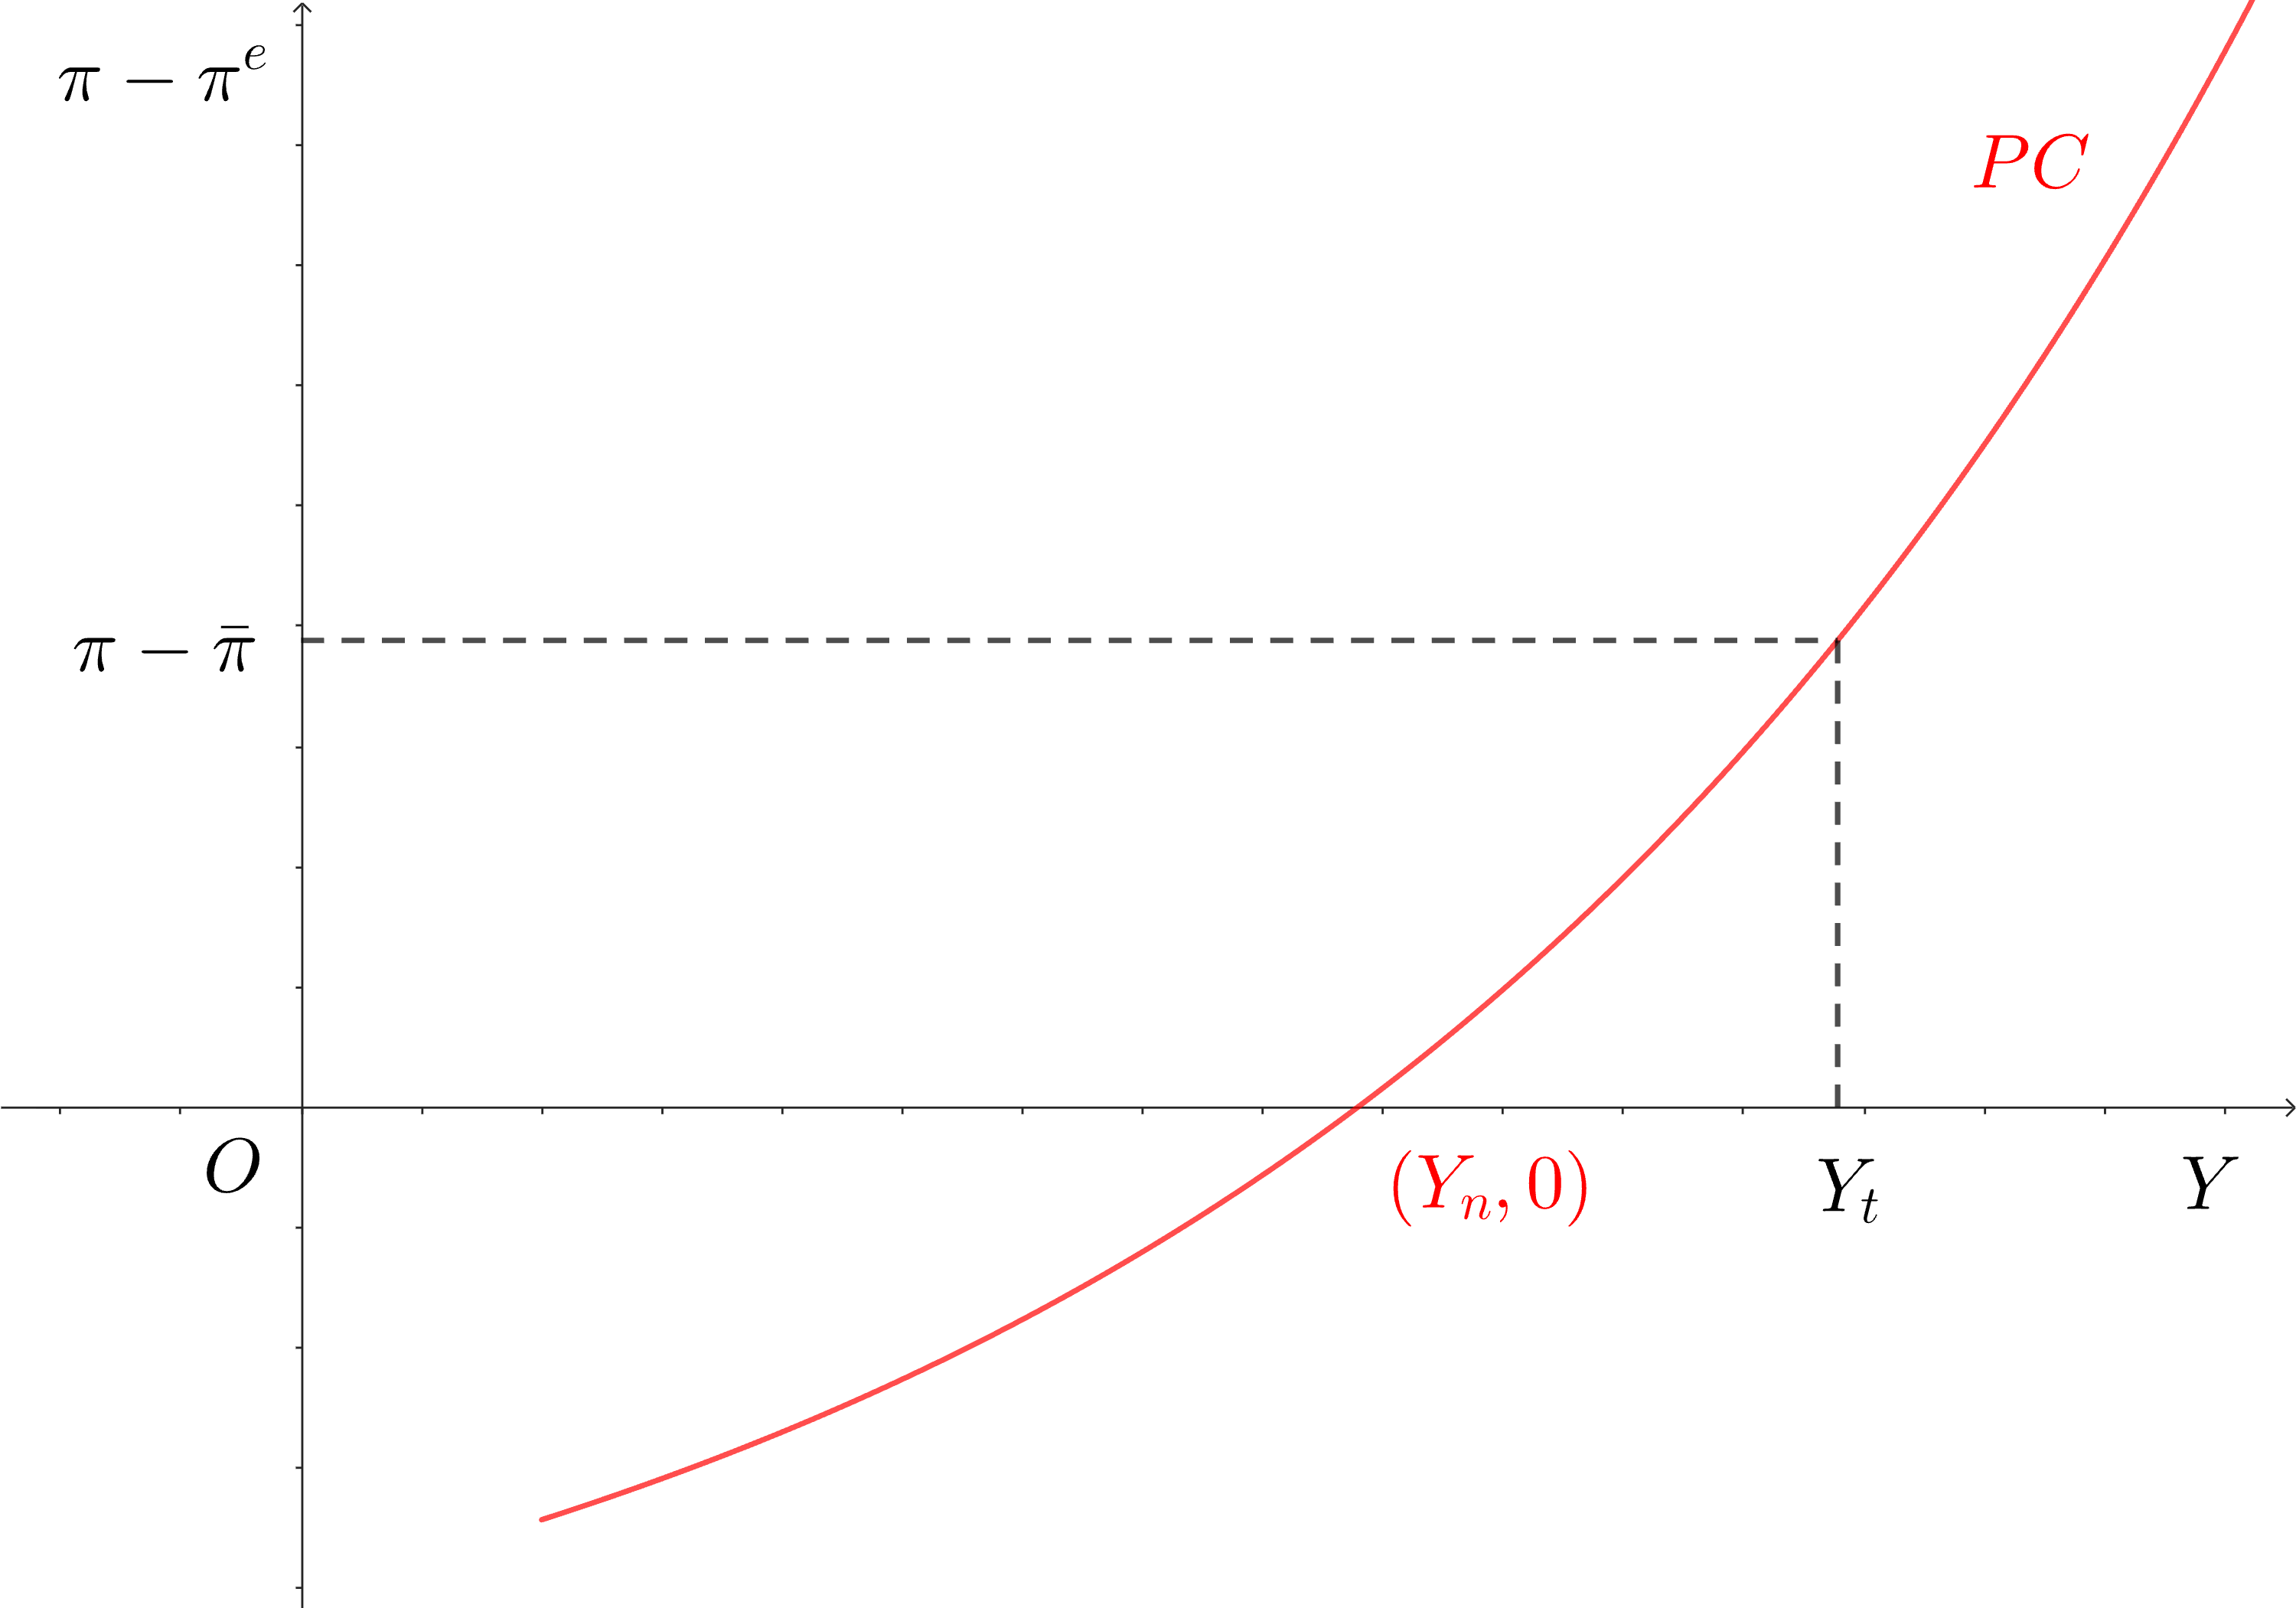
\includegraphics[width=0.6\textwidth]{pc01.png}
    \caption{PC Relation}
    \label{fig:pc01}
\end{figure}
\end{document}